\title{Study Guide for Midterm 1}
\author{Dr. Jordan Hanson - Whittier College Dept. of Physics and Astronomy}
\date{\today}
\documentclass[10pt]{article}
\usepackage[a4paper, total={18cm, 27cm}]{geometry}
\usepackage{outlines}
\usepackage{graphicx}
\usepackage{amsmath}
\begin{document}
\maketitle

\section{Chapter 1 - Introductory Concepts}
\begin{figure}[ht]
\centering
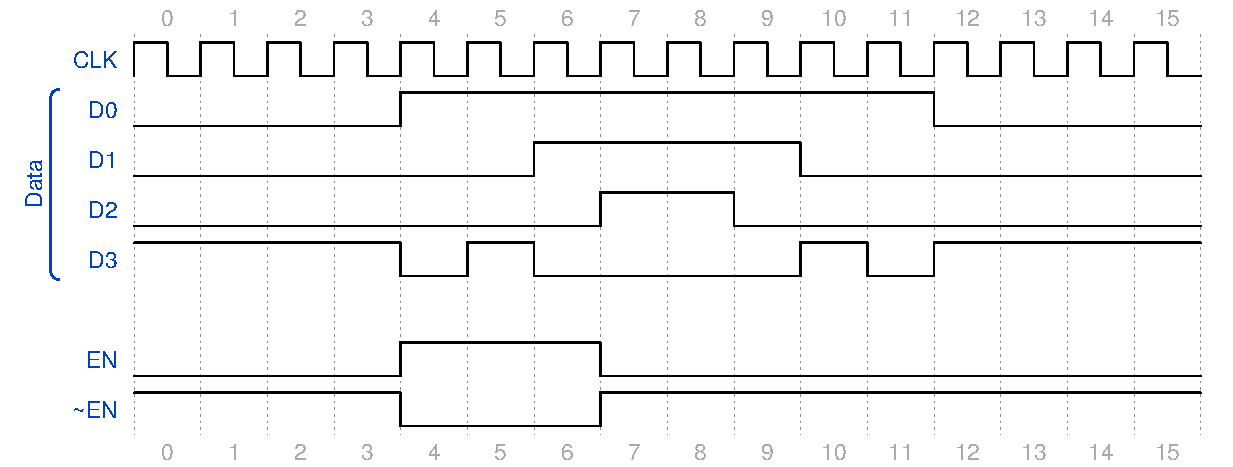
\includegraphics[width=0.75\textwidth]{timingExample1.pdf}
\caption{\label{fig:timing1} A timing diagram including a clock signal (CLK), a 4-bit parallel data stream (D0-D3), and enable/disable signals (EN/$\sim$EN).}
\end{figure}
\begin{enumerate}
\item Consider Fig. \ref{fig:timing1}. (a) If the clock frequency is 10 MHz, what is the period?  (b) What is the length of time represented in the waveform? (c) What is the length of the pulse in channel $D0$? \\ \\ 
\textit{(a) $0.1 \mu$s, (b) $1.6 \mu$s (c) $0.8 \mu$s.}
\item (a) What is the bit sequence represented by $D3$? (b) If $D0$ is a periodic signal, what is the duty cycle? \\ \\
\textit{(a) $1111010000101111$ (b) $50$\%.}
\item (a) Imagine that the four $D_i$ signals enter an AND gate, along with the EN signal.  Draw the resulting timing diagram. (b) Imagine that the four $D_i$ signals enter an AND gate, along with the $\sim$EN signal.  Draw the resulting timing diagram. \\ \\
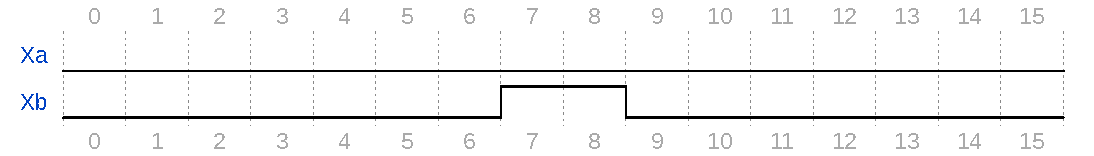
\includegraphics[width=0.9\textwidth]{timingExample4.pdf}
\item Suppose $D_i$ represents parallel data.  Each line gives 16 bits, and the clock frequency is 10 MHz.  (a) How many total bits are being sent across the $D_i$, and how long does it take?  What is the ratio of total bits to time?  (b) What would this time be if the data was transferred \textit{serially}, instead of in \textit{parallel}? \\ \\
\textit{(a) 64 bits, in $1.6 \mu$s, so the ratio is $40$ Megabits per second, (b) Four times as long, or 6.4 $\mu$s.}
\end{enumerate}

\section{Chapter 2 - Number Systems, Operations, and Codes}

\begin{enumerate}
\item Convert the following numbers to binary: (a) 33 (b) 65 (c) 129. (d) What does each number have in common? (e) Sketch a short python script to convert a decimal number to binary, and return the result. \\ \\
\textit{(a) $100001$ (b) $1000001$ (c) $10000001$ (d) Each number is one higher than a multiple of two, meaning the MSB and LSB are 1 with the rest of the digits being 0. (e)  }
\begin{verbatim}
DecimalToBinary(num):
        if num > 1: #1 in binary is just 1
            DecimalToBinary(num // 2) #Call recursively to get higher MSBs
            print num % 2 #If the number is divisible by current weight, 0, else 1
\end{verbatim}
\item Represent the following numbers in 8-bit binary: (a) -31 (b) -15 (c) -7.  (d) Show that each number, when added to its opposite is zero, in binary.  (e) Did you know that the \textit{shift} operators in C and Python can act as binary multipliers?  For example \verb+2 << 1+ results in 4.  Why? Because the code is saying $0010 \rightarrow 0100$. What is the result of the following codes in Python? 
\begin{verbatim}
j = 1
for i in range(0,5):
	print(j << i)	
\end{verbatim}
\textit{(a) $00001$, (b) $0001$, (c) $001$, (d) $11111+00001 = 1(00000)$, drop the MSB. Similarly, $1111+0001 = 1(0000)$, $111+001 = 1(000)$.}
\item What is the largest number that can be represented in binary with (a) $n = 4$ (b) $n = 8$ bits, if one bit must be used as a sign bit? \\ \\
\textit{(a) 15 (b) $127$ (The range is -128 to 127 including 0).}
\item Convert the following numbers to binary: (a) 0xFE (b) 0x7F (c) 0x3F. \\ \\
\textit{(a) $0xFE = 1111 1110$, (b) $0x7F = 0111 1111$ (c) $0x3F = 0011 1111$.}
\item Convert to hexadecimal: 1000100001000100 \\ \\
\textit{$0b1000 1000 0100 0100 = 0x8866$}
\item What is the following gray code sequence: 0011 0010 0111 0100 1110? \\ \\
\textit{$2...3...5...7...11$ (The first five prime numbers).}
\end{enumerate}

\section{Chapter 3 - Logic Gates}
\begin{figure}[ht]
\centering
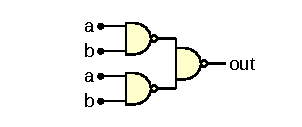
\includegraphics[width=0.3\textwidth]{gateExample1.pdf}
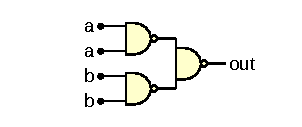
\includegraphics[width=0.3\textwidth]{gateExample2.pdf}
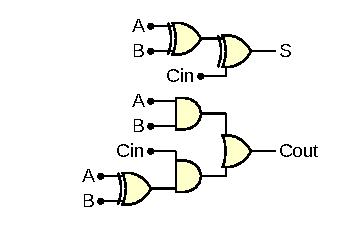
\includegraphics[width=0.3\textwidth]{gateExample3.pdf}
\caption{\label{fig:gates1} Examples of logic gate combinations.}
\end{figure}
\begin{enumerate}
\item Generate the truth tables for the gate diagrams in Fig. \ref{fig:gates1}. Pay attention to the domain.  \\ \\
\textit{(a) Like an AND gate:}
\begin{tabular}{| c | c | c |}
a & b & out \\
0 & 0 & 0 \\
0 & 1 & 0 \\
1 & 0 & 0 \\
1 & 1 & 1 \\
\end{tabular}
\textit{(b) Like an OR gate:}
\begin{tabular}{| c | c | c |}
a & b & out \\
0 & 0 & 1 \\
0 & 1 & 1 \\
1 & 0 & 1 \\
1 & 1 & 0 \\
\end{tabular}
\textit{(c) Like an:}
\begin{tabular}{| c | c | c | c | c |}
A & B & Cin & S & Cout \\
0 & 0 & 0 & 0 & 0 \\
0 & 0 & 1 & 1 & 0 \\
0 & 1 & 0 & 1 & 0 \\
0 & 1 & 1 & 0 & 1 \\
1 & 0 & 0 & 1 & 0 \\
1 & 0 & 1 & 0 & 1 \\
1 & 1 & 0 & 0 & 1 \\
1 & 1 & 1 & 1 & 1 \\
\end{tabular}
\item Identify the actions of the gate combinations in the previous problem from the truth tables.  (a) Fig. \ref{fig:gates1}, left: \textbf{AND gate} (b) Fig. \ref{fig:gates1}, middle: \textbf{OR gate} (c) Fig. \ref{fig:gates1}, right: \textbf{2-bit adder with carry}.
\item Suppose the signals in Fig. \ref{fig:timing2} are fed into the circuit in Fig. \ref{fig:gates1}, right.  Fill in the S and Cout signals in Fig. \ref{fig:timing2} \\ \\
\textit{See below in the figure.}
\begin{figure}[ht]
\centering
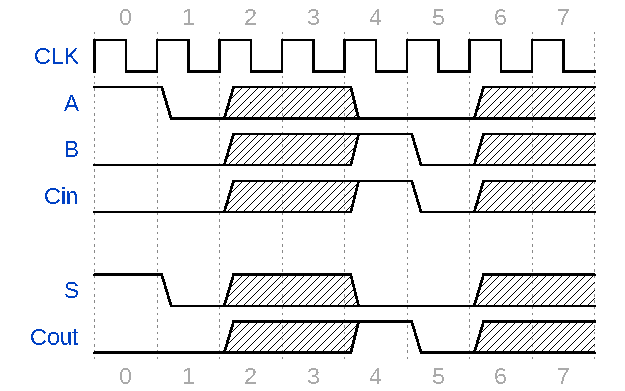
\includegraphics[width=0.5\textwidth]{timingExample5.pdf}
\caption{\label{fig:timing2} An example timing diagram for Fig. \ref{fig:gates1}, right.  The shaded regions indicate ``don't care'' conditions, or times when the data is not relevant.}
\end{figure}
\item Imagine a system for an electronic door lock which requires two electronic keys (two signals), S1 and S2.  The circuit has a red LED, a yellow LED, and a green LED.  The system unlocks when the output LOCK signal is LOW, caused by a LOW S1 and a LOW S2.  The red LED is activated when S1 and S2 are both HIGH.  The yellow LED is activated when S1 and S2 are different.  The green LED is activated when the system is unlocked.  \textit{By default, S1 and S2 are HIGH.} Draw the solution below.  \\ \\
\textit{Let S1 and S2 be the two signals.  They are by default HIGH signals.  They are fed into an OR gate.  The output of the OR gate is the Unlock signal UL.  A plain HIGH signal is connected to a resister and then to the green LED, which is connected to UL.  Thus, when both S1 and S2 go low (active low), then the green LED will be pulled down and on as UL goes LOW to unlock the lock.  S1 and S2 are connected in parallel to an AND gate, which powers a red LED and series resister with a HIGH output.  Finally, an XOR gate powers a resister and yellow LED when S1 and S2 are different.}
\end{enumerate}

\section{Chapter 4 - Boolean Algebra and Logic Simplification}
\begin{figure}[ht]
\centering
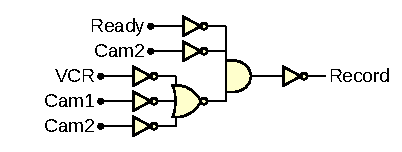
\includegraphics[width=0.4\textwidth]{gateExample4.pdf}
\caption{\label{fig:gates2} A gate combination triggering a signal named ``record.''}
\end{figure}
\begin{enumerate}
\item Consider the circuit in Fig. \ref{fig:gates2}.  (a) Write a logic expression for \textit{Record}. (b) Simplify the expression to as minimal a form as possible. (c) Are any signals or gates unnecessary? \\ \\
\textit{(a-b) The output record always evaluates to true:}
\begin{align}
\bar{Rec} &= \bar{R}\bar{C_2}\overline{(\bar{V}+\bar{C_1}+\bar{C_2})} \\
\bar{Rec} &= \bar{R}\bar{C_2}V C_1 C_2 \\
\bar{Rec} &= \bar{R}VC_1 (C_2 \bar{C_2}) = 0 \\
\bar{Rec} &= 0 \\
Rec &= 1
\end{align}
\textit{(c) What if we remove $C_2$?  Then the expression does not always evaluate to true $Rec = R + \bar{V} + \bar{C_1}$.}
\item Consider again the logic expression that represents the circuit in Fig. \ref{fig:gates2}. (a) Write the corresponding domain-4 Karnaugh map.  (b) Use the Karnaugh map to produce the S-POS expression and truth table. \\ \\
\textit{(a) This is a special case of the Karnaugh map: all boxes contain a 1, and the largest group is 16.  All variables are redundant, so the resulting expression is just TRUE.  (b) The truth table is trivial, and the S-POS expression is empty (cannot be written in standard form).}
\end{enumerate}

\section{Chapter 5 - Combinatorial Logic Analysis}
\label{sec:comb}
\begin{figure}[ht]
\centering
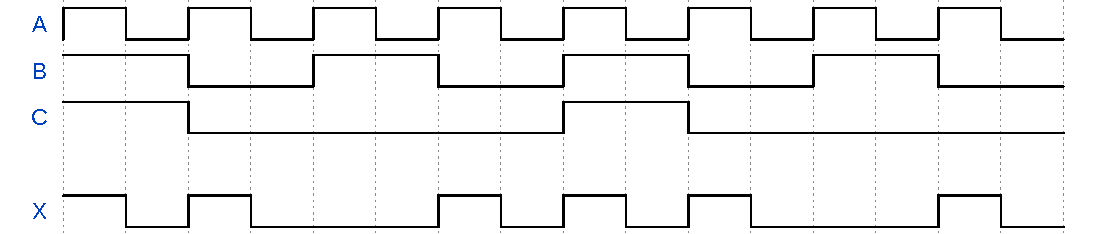
\includegraphics[width=0.5\textwidth]{timingExample3.pdf}
\caption{\label{fig:timing3} Timing diagram for Sec. \ref{sec:comb}.}
\end{figure}
\begin{enumerate}
\item (a) Draw the circuit corresponding to the timing diagram in Fig. \ref{fig:timing3}.  (b) Create the Karnaugh map.  (c) Using the Karnaugh map, write the simplest expression for this logic function and re-draw the circuit.\\ \\
\textit{(a) The circuit follows the expression $X = ABC + A\bar{B}C + A\bar{B}\bar{C}$.  It requires one OR gate and three 3-input AND gates.  (b) The Karnaugh map is the usual domain-3 map with two groups of two true states each.  (c) Using the Karnaugh map, the expression reduces to $X = A\bar{B} + AC$, which requires two 2-input AND gates and one 2-input OR gate.}
\end{enumerate}

\end{document}